\chapter{LITERATURE REVIEW}

\section{Introduction to LoRa}
\label{sec:LoRa}
% Sf, Bandwidth, Time on Air etc.
\subsubsection{Introduction}

\subsection{What is LoRa}
\label{sec:LoRa}

\hspace{12pt} In an era dominated by the \ac{IOT}, where countless devices are interconnected to enable smart and efficient systems, the need for robust, long-range, and low-power communication solutions has become paramount. LoRa (Long Range) technology emerges as a promising contender in fulfilling these requirements, offering a potent mix of long-distance coverage, low power consumption, and cost-effectiveness.\\

LoRa technology is a wireless communication protocol developed by Semtech Corporation, designed specifically to address the challenges of long-range communication with low power consumption, making it ideal for \ac{IOT} applications.

\subsubsection{Key Features of LoRa}
These are the key features that make LoRa stand out compared to other communication systems.

\begin{itemize}
    \item \textbf{Long Range:} LoRa technology is capable of transmitting data over several kilometers in urban environments and even greater distances in rural areas, making it suitable for applications requiring wide-area coverage.
    
    \item \textbf{Low Power Consumption:} LoRa devices are designed to operate on minimal power, enabling long battery life and prolonged device uptime. This makes LoRa technology ideal for \ac{IOT} devices deployed in remote or inaccessible locations.

    \item \textbf{Secure Communication:} LoRa employs advanced encryption techniques to ensure the confidentiality and integrity of transmitted data, protecting against eavesdropping and tampering.

    \item \textbf{Scalability:} LoRa networks can easily scale to accommodate thousands of devices, thanks to their decentralized architecture and efficient communication protocols.
\end{itemize}

\subsubsection{How Does LoRa Work}
\hspace{12pt} LoRa employs a unique modulation technique called Chirp Spread Spectrum (CSS), which enables it to achieve remarkable communication ranges while maintaining low power consumption. In CSS, data is encoded into chirp signals that gradually change frequency over time. This method allows LoRa devices to transmit data over long distances, even in environments with significant interference or obstacles.\\

Chirp stands for 'Compressed High Intensity Radar Pulse'. It is a signal which frequency either increase or decrease with time. It is also used in spread spectrum.

\begin{figure}[htp!]
    \centering
    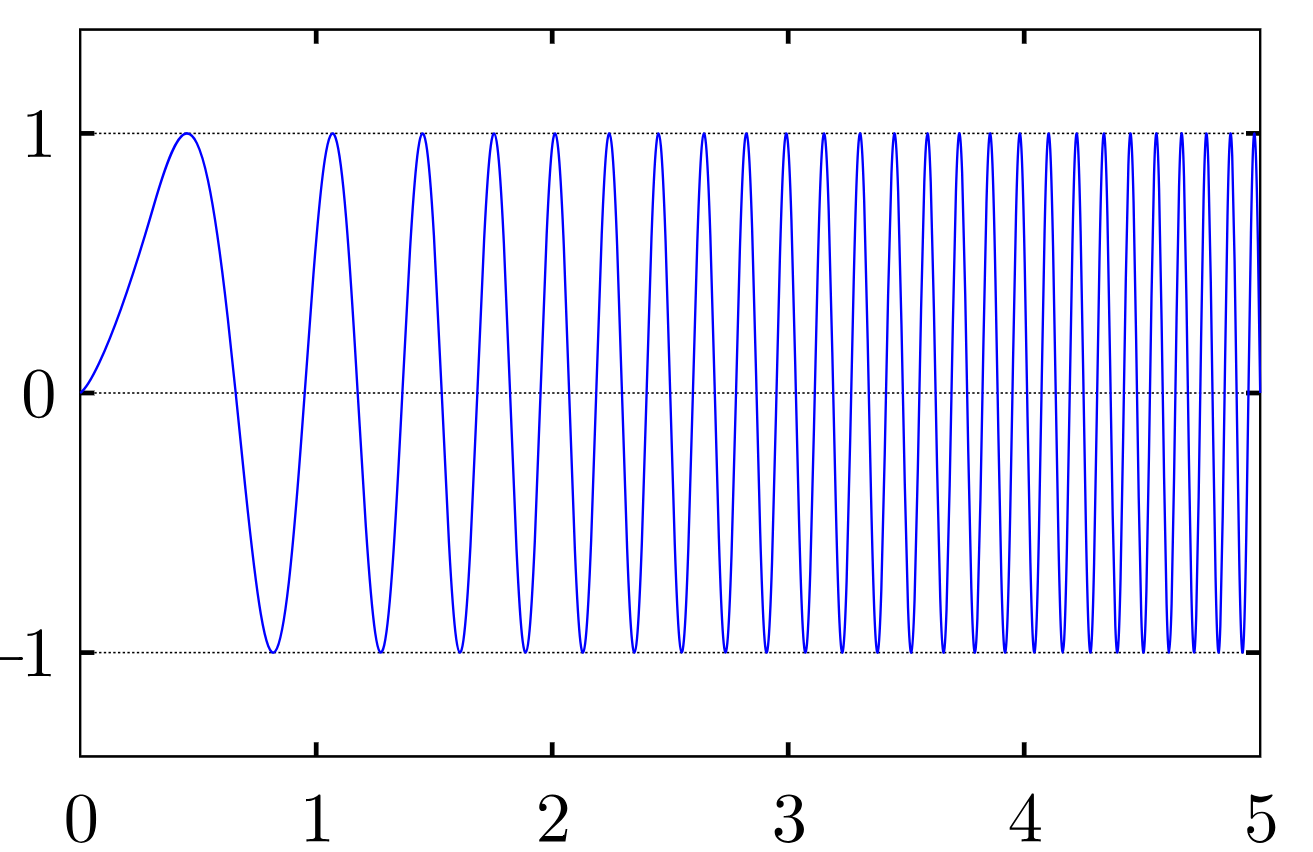
\includegraphics[scale=0.3]{images/Screenshot 2024-04-01 190918.png}
    \caption{Sinusoidal Chirp Wave Form}
\end{figure}

LoRa networks typically consist of two main components: LoRa end devices (nodes) and LoRa gateways. End devices are equipped with LoRa transceivers and sensors to collect and transmit data, while gateways serve as intermediate stations that receive data from end devices and forward it to the network server. The network server then processes and routes the data to the appropriate applications or services.

\subsubsection{Key Parameters of LoRa}

\hspace{12pt} LoRa technology operates with several key parameters that allow users to customize communication to suit specific needs. Some of the key parameters include:\\
\\
\textbf{\ac{SF}:}\\

In LoRa terms, the amount of spreading code applied to the original data signal is called the spreading factor. Spreading Factor is the main key parameter of the LoRa. LoRa modulation encompasses a total of 6 spreading factors, namely SF7 to SF12. These spreading factors play a crucial role in influencing various aspects, including transmission range, data rate, time-on-air, battery life, and receiver sensitivity. \\

\begin{figure}[htp!]
    \centering
    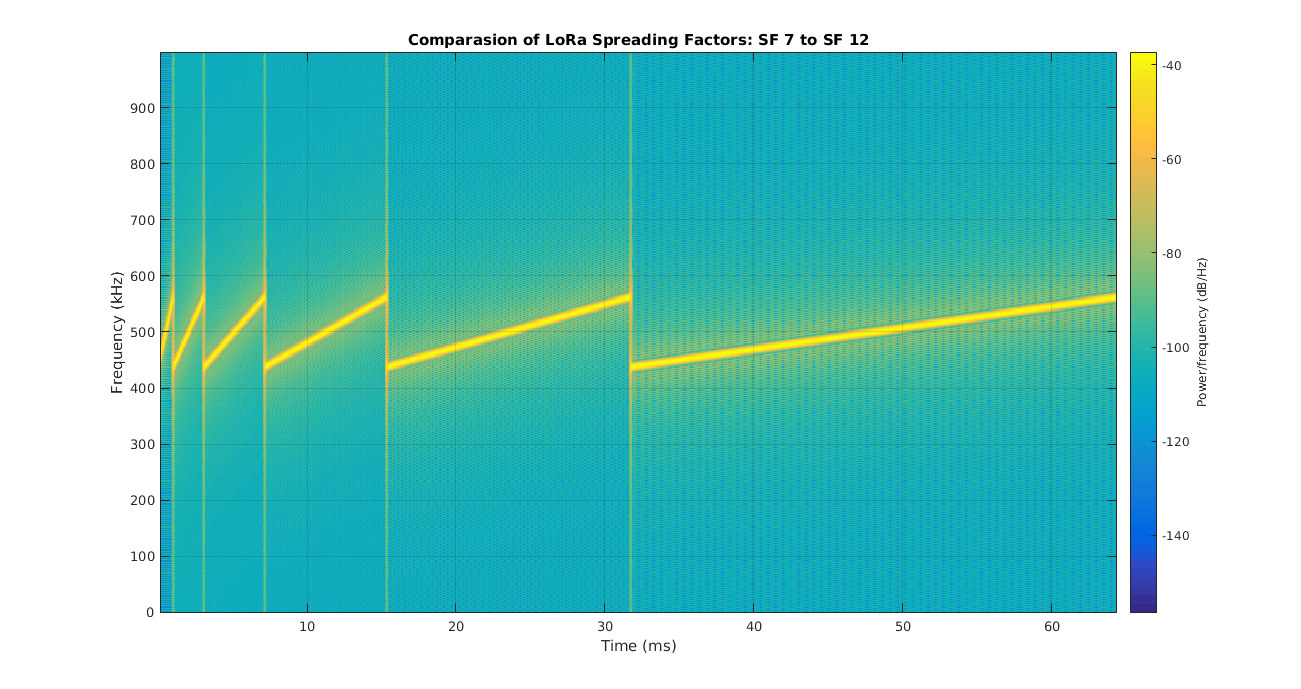
\includegraphics[scale=0.35]{images/SF_Comparasion_7_12.png}
    \caption{Comparison of \ac{SF}}
\end{figure}

The choice of spreading factor significantly impacts the communication parameters. Generally, using a larger spreading factor allows the signal to travel a greater distance and still be received without errors by the RF receiver. On the contrary, opting for a lower spreading factor provides a higher bit rate for a fixed bandwidth and coding rate. Larger spreading factors mean larger processing gain, and so a signal modulated with a larger spreading factor can be received with fewer errors compared to a signal with a lower spreading factor, and therefore travel a longer distance. Compared to a lower spreading factor, sending a fixed amount of data (payload) with a higher Spreading Factor and a fixed bandwidth needs longer time on air. Higher spreading factors provide higher receiver sensitivity. Usually, LoRa uses higher spreading factors when the signal is weak.\\

\begin{figure}[htp!]
    \centering
    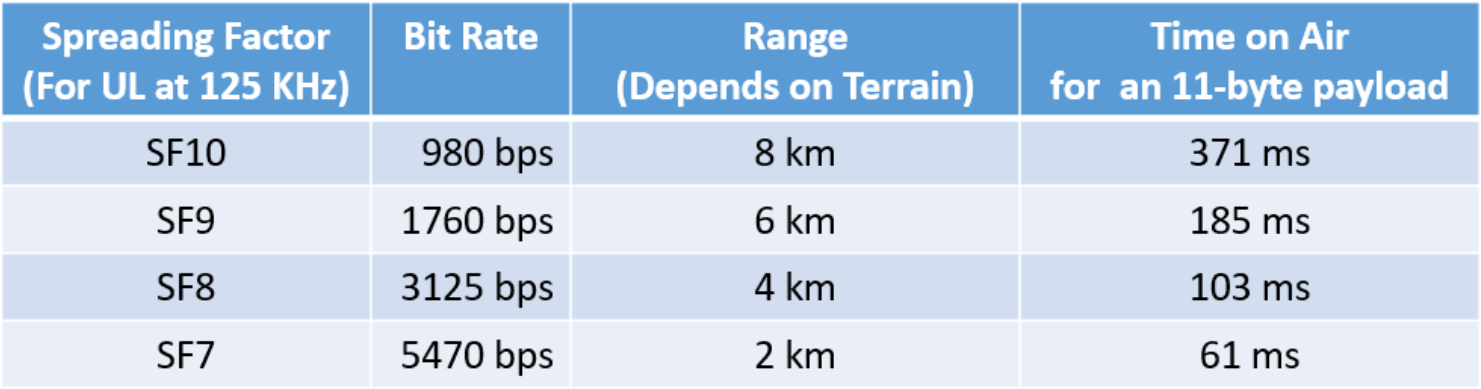
\includegraphics[scale=0.3]{images/sf with distance.png}
    \caption{Variation of Bit Rate, Range and \ac{ToA} with SF}
\end{figure}

\noindent\textbf{\ac{BW}:}\\

Bandwidth refers to the range of frequencies used for transmitting the signal. LoRa supports various bandwidth options, typically ranging from 125 kHz to 500 kHz. Wider bandwidths allow for higher data rates but may result in reduced range and increased power consumption.\\
\\
\textbf{\ac{CR}:}\\

The Code Rate of a forward error correction expresses the proportion of bits in a data stream that carries useful information. LoRa offers four different code rates: 4/5, 4/6, 4/7, and 4/8. For instance, in code rate 4/5, 4 bits convey useful data out of a total of 5 bits, where 1 bit serves as redundancy. The useful bit rate is determined by the following formula. \\
\\
\textbf{Output Power:}\\

Output Power determines the strength of the transmitted signal. It affects the communication range, with higher output power enabling a longer range but consuming more power.


\begin{figure}[htp!]
    \centering
    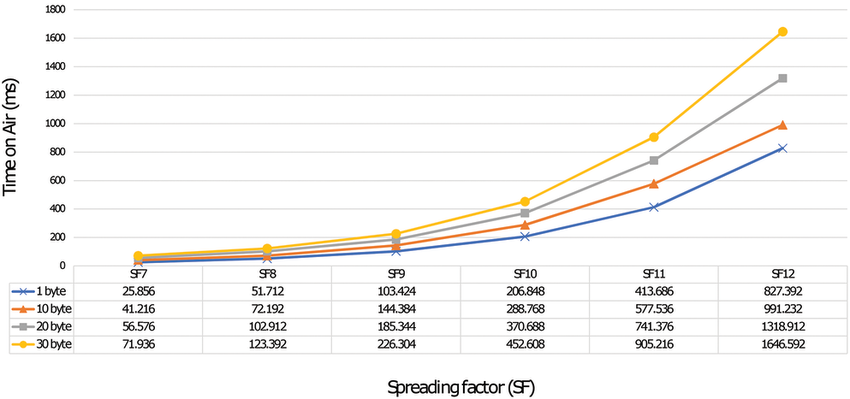
\includegraphics[scale=2]{images/LoRa-time-on-air-versus-SF-with-CD-4-5-and-125kHz-BW.png}
    \caption{ToA vs SF for BW=125kHz and CR=4/5}
\end{figure}

NEED TO ADD MORE PICTURES EXPLAINATION\\

\section{Research Findings}
\label{sec:Research}
\hspace{12pt} In our project, latency emerges as a critical concern. Despite extensive literature review, we encountered a notable absence of research or applications focusing on the latency aspect of LoRa, primarily because LoRa technology was originally designed to prioritize low bit rates, low power consumption, and long-range transmission.\\

In \cite{farooq}, a theoretical concept is briefly mentioned, suggesting that comparable range to the highest Spreading Factor (SF) can be achieved by employing three hops of the lowest SF, albeit with lower latencies. However, while this concept is introduced, its practical validation is lacking within their research.
